\begin{figure}[bt!]
	\begin{center}
		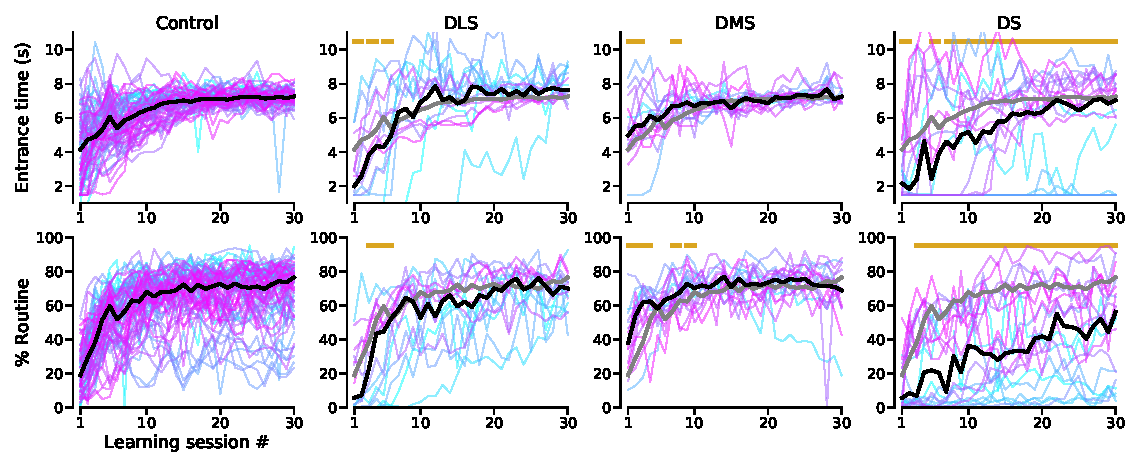
\includegraphics[width=\textwidth]{ch-lesion/figures/EarlyLesionLearning.pdf}
		\caption[Effect of Striatal Lesions on Learning]
		{\textbf{Learning the task is preserved in na\"{i}ve animals with striatal lesions.}
		\textbf{A)}
		Session-by-session improvement in performance for animals without lesion (control, \textit{first column}) and for animals that received a lesion prior to training (\textit{second to last columns}).
		Black lines indicate the control group median.
		Thin colored lines indicate single animals.
		Thick colored lines (same color code as in \autoref{fig:lesion:task}) in 3~rightmost columns indicate group performance for comparison (8 lesion animals with fewer than 30 training sessions are not shown, which explains the difference in the number of animals in this figure and in \autoref{fig:method:LesionSizeLocation}).
		Horizontal golden lines indicate significant differences between control and lesion groups (corrected for multiple comparisons).
		Notice that several animals with entire \gls{ds} lesions fail to improve their performance.
		\textbf{B)}
		Trajectories before and after extensive training (sessions \#1 and \#30) for two animals with large \gls{ds} lesions.
		Note that, after extensive practice, \textit{R238} was capable of performing the wait-and-run routine.
		Trajectory color code is the same as in \autoref{fig:lesion:task}.
		\textbf{C)}
		Percentage of trials in which animals remained in the front region of the treadmill (computed for sessions \#25 to \#30) versus their lesion size.
		}
		\label{fig:lesion:EarlyLesionLearning}
	\end{center}
\end{figure}